\chapter{Introduction à la transformée de Fourier}
\section{Dirac}
\begin{wrapfigure}[15]{r}{4.5cm}
\vspace{-5mm}
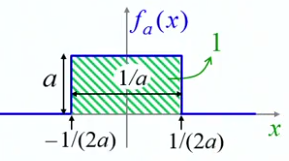
\includegraphics[scale=0.45]{ch1/image1.png}
\captionof{figure}{ }
\end{wrapfigure}
Nous allons commencer par l'étude de la distribution de Dirac, dernier grand 
physicien théoricien du 20$^e$ siècle, notamment en découvrant le positron, 
\dots Ici on va insister sur la \textit{distribution} que l'on peut voir comme 
une généralisation de la notion de fonction. Afin de l'introduire, étudions la 
fonction carrée (ou fenêtre) :


\begin{equation}
f_a(x) =\left\{\begin{array}{ll}
a &\text{ si } |x| \leq \frac{1}{2a}\\
0 &\text{ si } |x| > \frac{1}{2a}
\end{array}\right.
\end{equation}
donnant un carré de hauteur $a$ et de largeur $1/a$, sa surface vaut dès lors 
l'unité. 
\begin{equation}
\int_{-\infty}^\infty f_a(x)\ dx = 1
\label{eq:lim1}
\end{equation}
La distribution de dirac peut etre définie à partir de cette fonction 
en prenant la limite de $a$ tendant vers l'infini : sa hauteur tend vers 
l'infini tandis que sa largeur tend vers zéro.
\begin{equation}
\delta(x) = \lim\limits_{a\rightarrow\infty} f_a(x)
\end{equation}
On va appeler cette distribution $\delta(x)$ qui représente un pic placé en 
zéro, l'origine est le seul point ou l'on trouve une valeur particulière. On 
peut néanmoins dire que la surface sous la courbe vaut l'unité. Cela se 
voit à partir de \autoref{eq:lim1} : la surface sous la courbe ne dépend pas 
du paramètre $a$, d'où la surface unitaire :
\begin{equation}
\int_{-\infty}^\infty \delta(x)\ dx = 1
\end{equation}

\begin{wrapfigure}[7]{l}{4.5cm}
\vspace{-17mm}
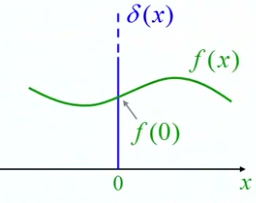
\includegraphics[scale=0.45]{ch1/image2.png}
\captionof{figure}{ }
\end{wrapfigure}
L'intérêt de cette distribution ne se remarque que par combinaison avec d'autres 
fonction. Considérons le produit d'une fonciton quelconque avec la fonction de 
Dirac. La seule fonction qui sera considérée est celle qui se trouve en zéro :
\begin{equation}
f(x)\delta(x) = f(0)\delta(x)
\end{equation}
Toutes les valeurs autres que celle de $x$ n'entre pas en ligne de compte. En 
intégrant ce produit 
\begin{equation}
\int_{-\infty}^{\infty} f(x)\delta(x)\ dx = \int_{-\infty}^\infty f(0)\delta(x)\ dx
= f(0)\int_{-\infty}^{\infty}\delta(x)\ dx = f(0)
\end{equation}
On voit que cette intégrale comme le "produit-scalaire" de $f$ avec $\delta$ qui 
sélectionne la valeur de la fonction à l'origine. En résumé
\begin{equation}
\delta(x) = \left\{\begin{array}{ll}
\infty & \text{ si } x = 0\\
0 & \text{ si } x \neq 0
\end{array} \right.
\end{equation}

\begin{wrapfigure}[7]{l}{4.5cm}
\vspace{-13mm}
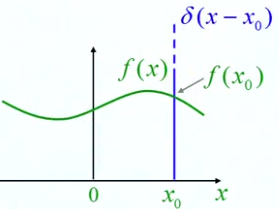
\includegraphics[scale=0.45]{ch1/image3.png}
\captionof{figure}{ }
\end{wrapfigure}
Cette notion peut être généralisée en déplaçant la distribution par translation en 
changeant l'argument $x$ en $x-x_0$ :
\begin{equation}
\delta(x-x_0) = \left\{\begin{array}{ll}
\infty & \text{ si } x=x_0\\
0 & \text{ si } x\neq x_0 
\end{array} \right.
\end{equation}
Cette distribution translatée multipliée par $f$ sélectionnera dès lors $f(x_0)$. 
La distribution de Dirac peut être définie par une infinité de fonction, tendant 
vers cette fameuse distribution lorsque le paramètre $a$ tend vers zéro. On peut 
par exemple prendre la distribution gaussienne 
\begin{equation}
\delta_a(x) = \frac{1}{a\sqrt{\pi}}e^{-x^2/a^2}  
\end{equation}
Lorsque $a$ tend vers zéro, on obtient un \textit{pic} tendant vers l'infini. On 
peut montrer que cette gaussienne, pour cette limite, tend bien vers la distribution 
de Dirac. Dans le cadre de ce cours, consacré à l'optique de Fourier, la distribution 
intéressante est la suivante
\begin{equation}
\delta_a(x) = \frac{1}{\pi x}\sin\left(\frac{x}{a}\right) = \frac{1}{2\pi}\int_{-1/a}^{1/a}
\cos(kx)\ dk
\end{equation}
Il s'agit d'une définition particulière, la suite du cours justifiera pleinement 
l'utilisation de celle-ci (les transformées de Fourier impliquent les fonction 
harmoniques). On va pouvoir trouver la distribution de Dirac à partir de
\begin{equation}
f(\alpha) = \int_{-\infty}^{\infty} \cos(\alpha x)\ dx
\end{equation}
La résultat dépendra de $\alpha$, ce résultat pourrait bien être une fonction de 
$\alpha$ qui se rapprochera très fortement de la distribution recherchée. Par 
intégration
\begin{equation}
f(\alpha) = \int_{-\infty}^{\infty} \cos(\alpha x)\ dx = \frac{1}{\alpha}\left[
\sin(\alpha x)\right]^\infty_{-\infty} = \frac{1}{a}[\sin(\infty)-\sin(-\infty)]
\end{equation}
Nous sommes face ici à une indétermination, cette intégrale généralisée n'est pas 
directement calculable. Il est préférable de travailler avec la fonction d'intégrale 
de Riemann aux bornes réelles pour ensuite faire tendre celle ci vers l'infini
\begin{equation}
\begin{array}{ll}
f(\alpha) = \int_{-L}^L \cos(\alpha x)\ dx &= \frac{1}{\alpha}[\sin(\alpha L)-\sin(-\alpha 
L)]\\
&= \frac{1}{\alpha}[\sin(\alpha L)+\sin(+\alpha L)]\\
&= 2\frac{\sin(\alpha L)}{\alpha}
\end{array}
\end{equation}

\begin{wrapfigure}[8]{r}{4.5cm}
\vspace{-5mm}
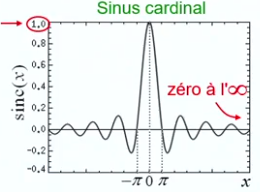
\includegraphics[scale=0.45]{ch1/image4.png}
\captionof{figure}{ }
\end{wrapfigure}
Considérons l'artifice mathématique suivant, permettant de faire apparaître le 
sinus cardinal ($\equiv \sin x/x$) :
\begin{equation}
\begin{array}{ll}
f(\alpha) &= 2L \frac{\sin(\alpha L)}{\alpha L}\\
&= 2L\text{sinc}(\alpha L)
\end{array}
\end{equation}
La fonction sinus cardinal tend vers zéro à l'infini, il s'agit d'une fonction paire dont 
la valeur à l'origine vaut l'unité (valeur donnée par la levée de l'indétermination). Cette 
fonction à des zéros multiples que l'on retrouve à chaque multiple de $\pi$.\newpage

\begin{wrapfigure}[8]{l}{4.5cm}
%\vspace{-5mm}
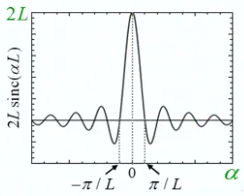
\includegraphics[scale=0.45]{ch1/image5.png}
\captionof{figure}{ }
\end{wrapfigure}
Revenons à nos moutons. Notre fonction sinus cardinal à pour argument $\alpha L$ : les zéros 
de la fonction d'origines se voient tous divisés par $L$ et l'ordonnée à l'origine vaut $2L$. 
Une fois que $\alpha$ n'est plus nul, on redescend brusquement vers un premier zéro (les 
oscillations se comprennent très facilement en interprétant l'aire sous la courbe en faisant 
augmenter $\alpha$).\\
\ \\

\begin{wrapfigure}[8]{r}{7.5cm}
\vspace{-15mm}
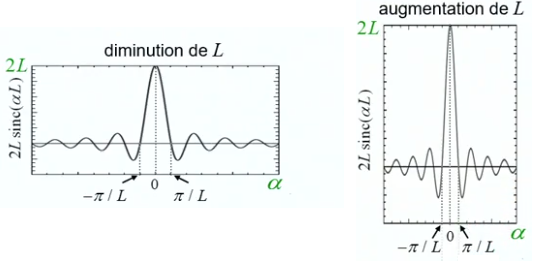
\includegraphics[scale=0.45]{ch1/image6.png}
\captionof{figure}{ }
\end{wrapfigure}
Intéressons nous ce qui se passe lorsque $L \rightarrow \infty$. Remarquons premièrement 
qu'une diminution de $L$ correspond à un \textit{aplatissement} et \textit{élargissent} du 
graphe. Inversement, lorsque $L$ augmente elle gagne en hauteur et les zéros se rapprochent 
de l'origine. Que devient cette fonction pour $L \rightarrow\infty$ ? Montrons que l'on 
obtient, à un facteur près, la distribution de Dirac 
\begin{equation}
f(a) = \lim\limits_{L\rightarrow\infty} \int_{-L}^L \cos(\alpha x)\ dx = \lim\limits_{L 
\rightarrow \infty}[2L\text{sinc}(\alpha L)]
\end{equation}
Cette limite n'est pas facile à appréhender, l'étude du graphe n'est pas fort utile. A 
défaut, on peut s'itnéresser à la surface du graphe de cette fonction en étudiant l'aire 
sous la courbe du sinus cardinal :
\begin{equation}
\int_{-\infty}^\infty \text{sinc }(\alpha x)\ dx = \int_{-\infty}^\infty \dfrac{\sin(\alpha
x)}{\alpha x}\ dx = \dfrac{\pi}{a}
\label{eq:AireD}
\end{equation}
\danger Il ne faut pas confondre la variable $\alpha$ avec celle d'intégration, $x$. Nous 
montrons ici que $f(\alpha)$ peut être associée à la distribution. Dans \autoref{eq:AireD} 
remplaçons $x$ par $\alpha$ par "l'ancien $\alpha$ jouera le rôle du paramètre $L$ :
\begin{equation}
\int_{-\infty}^\infty \text{sinc }(L\alpha)\ d\alpha = \int_{-\infty}^\infty \dfrac{\sin(L\alpha)
}{L\alpha}\ d\alpha = \dfrac{\pi}{L}
\end{equation}
En multipliant par $2L$ (pouvant directement rentrer dans l'intégrale):
\begin{equation}
\int_{-\infty}^\infty2L \text{sinc }(L\alpha)\ d\alpha = \int_{-\infty}^\infty \dfrac{\sin(L\alpha)
}{L \alpha}\ d\alpha = 2\pi
\end{equation}
Cette surface vaut $2\pi$, mais ce qui est important est que celui-ci est indépendant 
du paramètre $L$ exactement comme on l'avait pour la fonction fenêtre avec l'aire unitaire ; 
faire tendre $L$ vers l'infini ne change dès lors rien. Les caractéristiques sont celles de 
la fonction de Dirac. Pour retrouver cette distribution, il nous suffit de diviser par $2\pi$.
\begin{equation}
\int_{-\infty}^\infty \lim\limits_{L\rightarrow\infty}[\frac{2L}{2\pi}\text{sinc}(\alpha L)]\ 
d\alpha = \frac{2\pi}{2\pi}=1
\end{equation}
On peut ainsi assimiler ce résultat à la distribution de Dirac :
\begin{equation}
\text{Distribution de Dirac : } \delta(\alpha) = \lim\limits_{L\rightarrow\infty}\left[
\dfrac{L}{\pi}\text{sinc}(\alpha L)\right]
\end{equation}
Cette fonction est \textit{piquée} à l’origine et une largeur tendant vers zéro dont l'aire
sous la courbe faut bien 1. On peut dès lors écrire
\begin{equation}
f(a) = \lim\limits_{L\rightarrow\infty} \int_{-L}^L \cos(\alpha x)\ dx = \lim\limits_{L 
\rightarrow \infty}[2L\text{sinc}(\alpha L)] = 2\pi \delta(\alpha)
\end{equation}
Sous la forme d'une intégrale généralisée, résultat pratique pour l'étude des transformées 
de Fourier.
\begin{equation}
\int_{-\infty}^\infty \cos(\alpha x)\ dx = 2\pi \delta (\alpha)
\end{equation}
Notons qu'il n'est pas nécessaire de déterminer précisément ce que vaut $\alpha$, la 
"définition" ci-dessous est auto-suffisante
\begin{equation}
\int_{-\infty}^\infty f(\alpha)\delta(\alpha)\ d\alpha = f(0)
\end{equation}
Généralisons quelque peu ce que nous venons de faire en vue de passer à la transformée de 
Fourier. La notion de phaseur, exponentielle imaginaire est fondamentale :
\begin{equation}
\int_{-\infty}^\infty e^{i\alpha x}\ dx = \int_{-\infty}^\infty \cos(\alpha x)\ dx + i
\int_{-\infty}^\infty \sin(\alpha x)\ dx
\end{equation}
Cette exponentielle imaginaire cache la fonction $cos(\alpha x)$ que nous venons d'étudier 
avec en plus une partie imaginaire. Que vaut la contribution de la partie imaginaire ? 
\begin{equation}
\int_{-L}^L \sin(\alpha x)\ dx = -\frac{1}{\alpha}\left[\cos(\alpha x)\right]^L_{-L} = 0
\end{equation}
Il n'est même pas ici nécessaire de faire tendre $L\rightarrow\infty$, le cosinus étant 
une fonction paire cela donne tout simplement zéro (directement visible, car l'intégration 
d'une fonction impaire aux bornes centrées sur zéro est identiquement nulle). \\
En conclusion:
\begin{equation}
\dfrac{1}{2\pi}\int_{-\infty}^\infty e^{i\alpha x}\ dx  = \delta(\alpha)
\end{equation}

\newpage
\section{Transformée de Fourier : introduction}






































